\section{Stochastic processes}

\begin{definition}[\textit{Stochastic process}]
    A stochastic process is an infinite sequence of random variables that is contingent upon the outcomes of a random experiment.
\end{definition}
Thus, a stochastic process can be represented by the function:
\[v(t)=\varphi(s,t)\]
Here, $s$ denotes the outcome of a random experiment, and $t$ represents the corresponding time.

\begin{definition}[\textit{Realization}]
    A specific instance $v(t) = \varphi(\bar{s}, t)$ is termed a realization of the process.
\end{definition}
\begin{figure}[H]
    \centering
    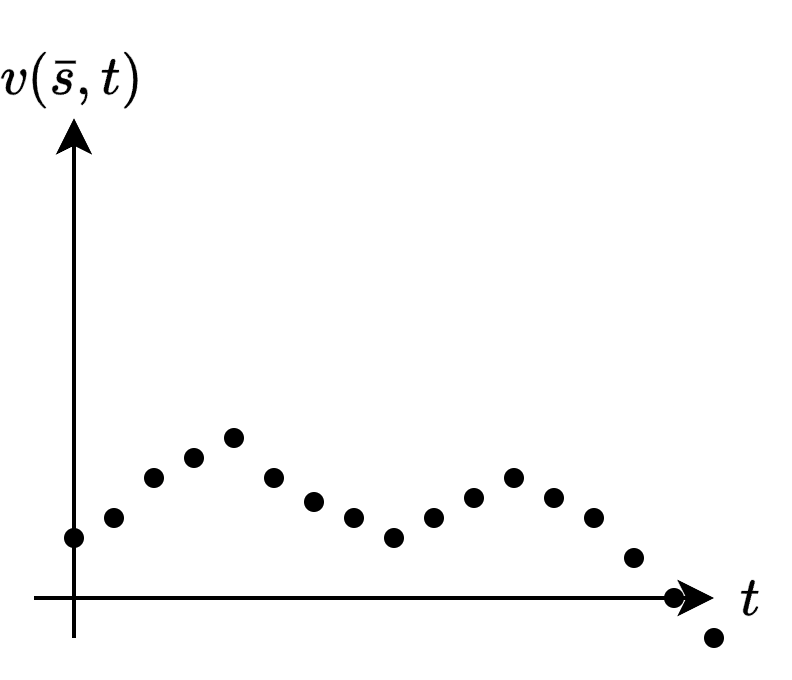
\includegraphics[width=0.25\linewidth]{images/outcome.png}
    \caption{Visual representation fixed outcome}
\end{figure}
If instead of fixing the outcome of the experiment, we constrain the value of time, multiple outcomes can occur simultaneously at that time instant.
\begin{figure}[H]
    \centering
    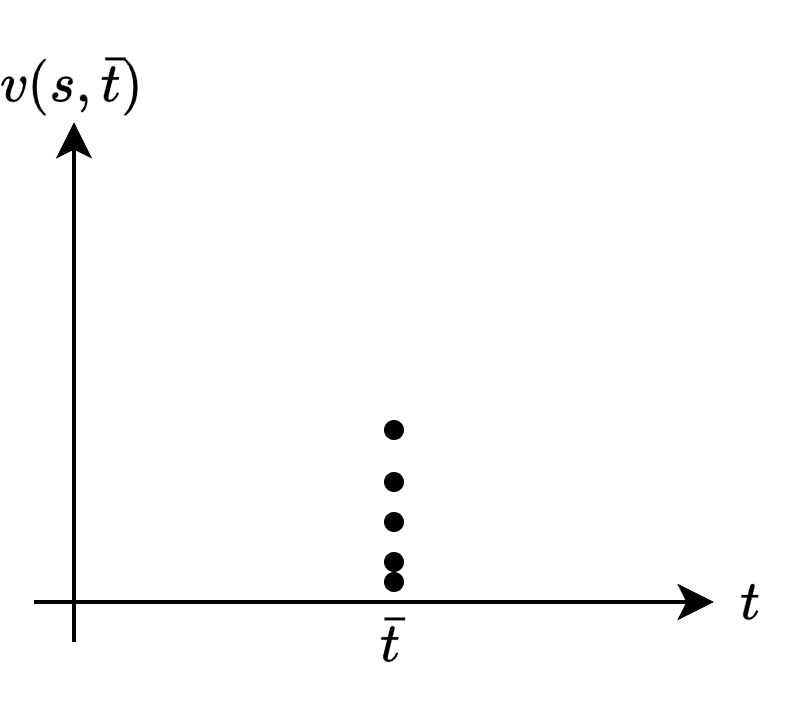
\includegraphics[width=0.25\linewidth]{images/time.png}
    \caption{Visual representation fixed time}
\end{figure}

For any positive integer $n$ and any $n$-tuple of instants $t_1, t_2, \dots, t_n$, we can characterize $v(t_1), v(t_2), \dots, v(t_n)$ as follows:
\[F_{t_1,t_2,\dots,t_n}(q_1,q_2,\dots,q_n)=\text{P}\left(v(t_1)<q_1,v(t_2)<q_2,\dots,v(t_n)<q_n\right)\]
However, specifying all the $q_i$ values in practice is often too complex, rendering this method impractical.

\subsection{Covariance}
Consider various realizations $s_1, s_2, \dots, s_n$ stemming from a specific experiment. 
The expected value signifies the average across all potential realizations at each time instance $\bar{t}$.
Extending this concept across infinite time instants yields the expected value $\mu(t)$:
\[\mu(t)=\mathbb{E}\left[ v(t) \right]\]
This framework enables a comparison of $\mu$ values across distinct times $t_1$ and $t_2$. 
Such comparisons prove beneficial in predictive scenarios since leveraging historical data enhances accuracy.
Comparison across different time instances can be facilitated using the auto-covariance function:
\[\gamma(t_1,t_2)=\mathbb{E}\left[ \left(v(t_1)-\mu(t_1)\right) \cdot \left(v(t_2)-\mu(t_2)\right) \right]\]
Here, the terms $v(t_1) - \mu(t_1)$ and $v(t_2) - \mu(t_2)$ represent deviations from the respective mean values $\mu(t_1)$ and $\mu(t_2)$.
A large variance suggests significant disparity among realizations.
When the two time instances coincide, i.e., $t = t_1 = t_2$, the equation simplifies to:
\[\gamma(t,t)=\mathbb{E}\left[ \left(v(t)-\mu(t)\right)^2 \right]\]
This expression corresponds to the variance of the variable $v(t)$ with itself. 

It's worth noting that variance is always non-negative, and its square root is referred to as the standard deviation $\sigma$:
\[\sigma(t)=\sqrt{\mu(t)}\] 
Additionally, the following relation holds:
\[\left\lvert \text{Cov}\left[v(t_1),v(t_2)\right] \right\rvert \leq \sqrt{\text{Var}\left[ v(t_1) \right]} \cdot \sqrt{\text{Var}\left[ v(t_2) \right]}\]
\begin{proof}
    Let's consider the realization of the function $v(t)$ at two time instants $t_1$ and $t_2$ as a vector  $v(t)=\begin{bmatrix} v(t_1) & v(t_2) \end{bmatrix}^T$. 
    The variance of this vector is defined through a vector-vector product as follows:
    \[\text{Var}\left[v\right]=\mathbb{E}\left[
    \begin{bmatrix}
        \left(v(t_1) - \mu (t_1)\right) \\ \left(v(t_2) - \mu(t_2)\right)
    \end{bmatrix}
    \begin{bmatrix}
        \left(v(t_1) - \mu (t_1)\right) & \left(v(t_2) - \mu(t_2)\right)
    \end{bmatrix} \right]\]
    Upon performing the multiplication, we obtain:
    \[\text{Var}\left[v\right] = 
    \begin{bmatrix}
        \mathbb{E}\left[ \left( v(t_1)-\mu(t_1) \right)^2 \right] & \mathbb{E}\left[ \left( v(t_1)-\mu(t_1) \right)\left( v(t_2)-\mu(t_2) \right) \right] \\
        \mathbb{E}\left[ \left( v(t_1)-\mu(t_1) \right)\left( v(t_2)-\mu(t_2) \right) \right] & \mathbb{E}\left[ \left( v(t_2)-\mu(t_2) \right)^2 \right] \\
    \end{bmatrix}\]
    In other words:
    \[\text{Var}\left[v\right] = 
    \begin{bmatrix}
        \text{Var} \left(v(t_1)\right) & \text{Cov}\left[v(t_1),v(t_2)\right] \\
        \text{Cov}\left[v(t_1),v(t_2)\right] & \text{Var} \left(v(t_2)\right) \\
    \end{bmatrix}\]
    The determinant of this matrix must be non-negative, implying:
    \[\text{Var} \left(v(t_1)\right) \cdot \text{Var} \left(v(t_2)\right) - \text{Cov}\left[v(t_1),v(t_2)\right]^2 \geq 0\]
    From this inequality, we can derive the initial formula.
\end{proof}
The covariance is a valuable tool for comparing two distinct processes, leading to the concept of cross-covariance.

\paragraph*{Normalized covariance function} 
The normalized covariance function, also known as the Pearson correlation coefficient, is defined as:
\[\rho(t_1,t_2)=\dfrac{\gamma(t_1,t_2)}{\sqrt{\gamma(t_1,t_1)} \cdot \sqrt{\gamma(t_2,t_2)}}\]
The absolute value of this function is always less than or equal to one:
\[\left\lvert \rho(t_1,t_2) \right\rvert \leq 1\]
Moreover, when considering the same time instant, i.e., $t = t_1 = t_2$, the normalized covariance function equals one.

\subsection{Correlation}
We can also compare values at different time instants using the auto-correlation function:
\[\tilde{\gamma}(t_1,t_2)=\text{Corr}\left[v(t_1),v(t_2)\right]=\mathbb{E}\left[ v(t_1) \cdot v(t_2) \right]\]
The correlation bears a relation to the covariance:
\[\gamma(t_1,t_2)=\tilde{\gamma}(t_1,t_2) - \mu(t_1)\mu(t_2)\]
\begin{proof}
    The formula can be derived as follows: 
    \begin{align*}
        \gamma(t_1,t_2) &= \mathbb{E}\left[ \left(v(t_1)-\mu(t_1)\right)\left(v(t_2)-\mu(t_2)\right) \right] \\
                        &= \mathbb{E}\left[ v(t_1)v(t_2)-\mu(t_1)v(t_2)-v(t_1)\mu(t_2)+\mu(t_1)\mu(t_2) \right] \\
                        &= \mathbb{E}\left[v(t_1)v(t_2)\right] -\mu(t_1)\mathbb{E}\left[v(t_2)\right]-\mu(t_2)\mathbb{E}\left[v(t_1)\right]\mu(t_2)+\mu(t_1)\mu(t_2) \\
                        &= \tilde{\gamma}(t_1,t_2) - \mu(t_1)\mu(t_2) - \mu(t_1)\mu(t_2) + \mu(t_1)\mu(t_2) \\ 
                        &= \tilde{\gamma}(t_1,t_2) - \mu(t_1)\mu(t_2)
    \end{align*}
    In the second step, we removed the mean values $\mu(t)$ since they are not random variables.
    Also note that by definition, $\mathbb{E}\left[v(t_1)\right] = \mu(t_1)$ and $\mathbb{E}\left[v(t_2)\right] = \mu(t_2)$.
\end{proof}
The correlation can also be used to compare two different processes, resulting in a cross-correlation.